\documentclass[a4wide,10pt]{scrartcl}
\usepackage[utf8]{inputenc}
\usepackage{amsmath,amssymb}
\usepackage{graphicx}
\usepackage{caption}
\usepackage{subcaption}

\newcommand{\Dt}{\Delta t}

% Title Page
\title{HPX \& odeint -- dataflow-driven ODE integration}
\author{}


\begin{document}
\maketitle

Suppose you need to find a numerical solution of an initial value problem (IVP) of an ordinary differential equation (ODE) given by:
\begin{equation}
 \dot{\vec x}(t) = \vec f(\vec x(t), t), \qquad \vec x(t=0) = \vec x_0.
\end{equation} 
Here, $\vec x \in \mathbb{R}^N$ is the state variable in the $N$-dimensional configuration space.
To find an approximation of the trajectory $\vec x(t)$ one first introduces a time discretization with some small step size $\Delta t$.
The numerical trajectory is then given by a sequence of points $\vec x_n$ that approximate the true trajectory at the points $t_n=n\cdot \Dt$, hence: $\vec x_n\approx\vec x(t_n)$.
The most simple, and also most common class of methods are the so called explicit single-step methods, which includes the Runge-Kutta methods, for example.
A single step method consists of a mapping $G(\Dt)$ that calculates the next point of the trajectory $\vec x_{n+1}$ only using one previous approximation $\vec x_n$ and a step-size $\Dt$:
\begin{equation}
 \vec x_{n+1} = G(\Dt) \vec x_n.
\end{equation}
Exemplarily, for the most trivial Euler method the mapping $G_\Dt$ is defined as:
\begin{equation}
 G(\Dt):\, \vec x_{n+1} = \vec x_n + \Dt \vec f(\vec x_n,t_n).
\end{equation}
The Euler method has order 1 only, which means the error of the numerical approximation has the order 2, thus $|x(\Dt) - x_1|\sim \Dt^2$.
Typically, one requires more accuracy and thus relies on methods with higher order.
The most important class of higher order schemes are the Runge-Kutta methods. 
These methods consist of $s$ stages where the rhs of the ODE is evaluated.
The mapping $G$ for a generic Runge-Kutta scheme with $s$ stages writes as:
\begin{equation}
 \begin{aligned}
    G_\Dt:\, \vec x_{n+1} &= \vec x_n + \Dt \sum_{k=1}^{s} b_k \vec y_k \\
    \text{where}\quad \vec y_k &= f( \vec x_n + \Dt \sum_{m=1}^k a_{k,m} \vec y_m , t_n+c_k\Dt).
   \end{aligned}
\end{equation}
The parameter sets $a_{k,m}$, $b_k$ and $c_k$ have to be chosen such that the result $x_{n+1}$ is indeed an approximation of some order $p$.
We note that for simplicity we here restrict the study to methods with constant step-size~$\Dt$, but the method below can also be applied to embedded Runge-Kutta schemes required for step size control.
To obtain an approximation of a whole trajectory from $t=0\dots t_\text{end}$ one applies the above one-step algorithm subsequently to obtain a descretized approximate trajectory $\vec x_0,\vec x_1,\vec x_2,\dots,\vec x_T$ with $T=t_\text{end}/\Dt$.

Trying to parallelize the algorithm one immediately realizes that no two time steps can be computed in parallel because of its dependence on the previous state.
So no parallelization in the time domain is possible and one has to compute the trajectory points one by one: $\vec x_0\rightarrow\vec x_1 \rightarrow \vec x_2 \dots$.
However, given a high dimensional system one can divide the state $\vec x$ into regions and thus distribute the work on many cores/processors/machines.

We compare the performance of OpenMP (OMP) with an HPX dataflow (HPX df) and HPX local dataflow (HPX ldf) implementation.
The benchmark is a 2D lattice simulation with $N\times N$ sites where $N=512,1024,2048$.
We first study the influence of the granularity on the run-time, and then analyze the strong scaling on two machines: a 2 processor, 16 Core Intel Xeon machine and a 4 processor, 64 Core Opteron unit.

For the OMP runs we used GOMP\_CPU\_AFFINITY and OMP\_PROC\_BIND to pin the OMP threads to specific cores.
Furthermore, for runs that did not occupy all available cores we checked several thread distributions (single NUMA domain vs more available Cache) to find the optimal core allocation.

We find that HPX is more sensitive to the granularity, which in our simulation is the number of rows per task.
Especially the dataflow implementation (HPX df) needs to be run with exactly the right granularity to give optimal performance.
If there is not enough work available, the overhead of the HPX dataflow threads overtakes the gain from additional cores and reduces the performance, see Fig.~\ref{fig:granularity_32}.
Using local dataflows, this can be avoided because much less overhead is introduced in local dataflows.

\begin{figure}
 \begin{subfigure}[b]{0.49\textwidth}
  \centering
  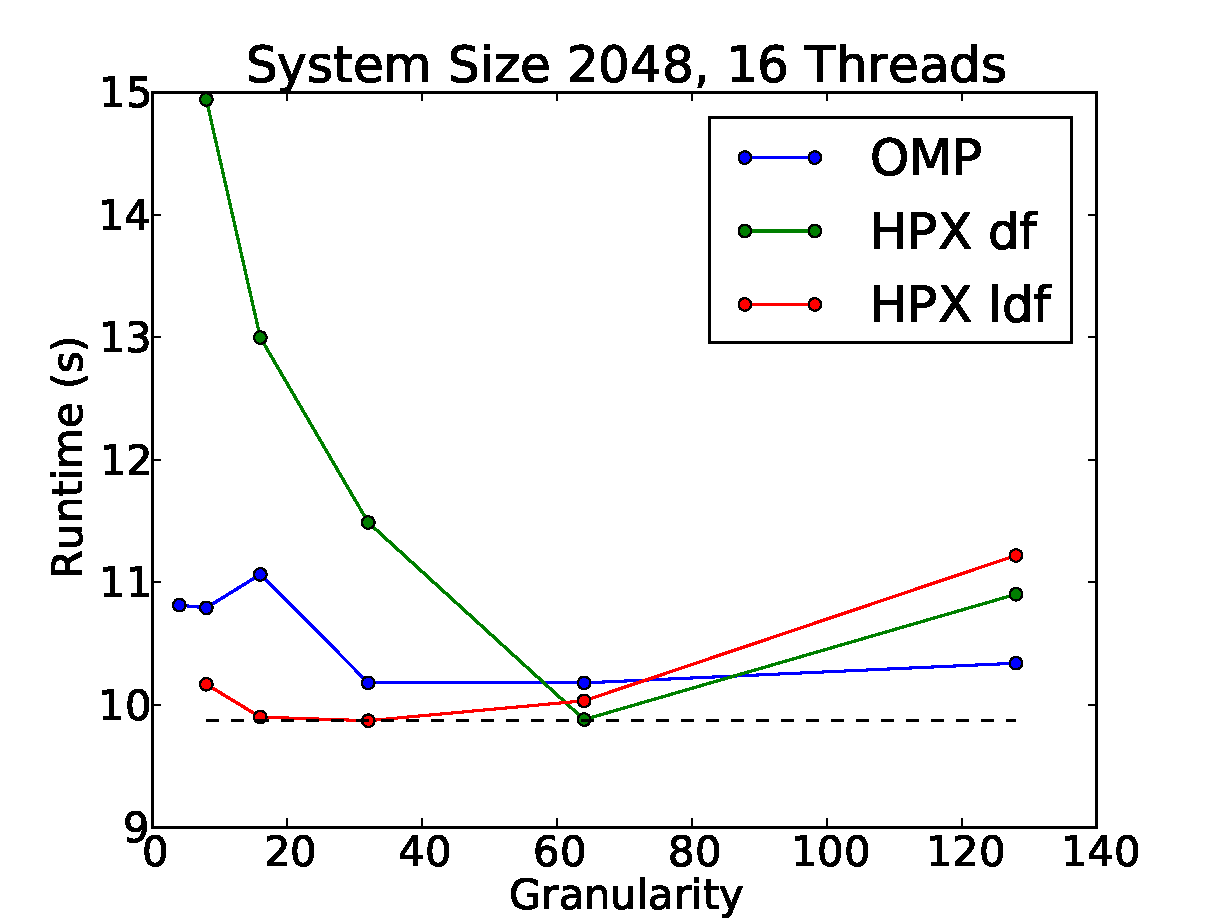
\includegraphics[width=\textwidth]{../plot/trillian_granularity_16.pdf}\hfill
  \caption{Granularity with 16 Threads.} 
  \label{fig:granularity_16}
 \end{subfigure}
 \begin{subfigure}[b]{0.49\textwidth}
  \centering
  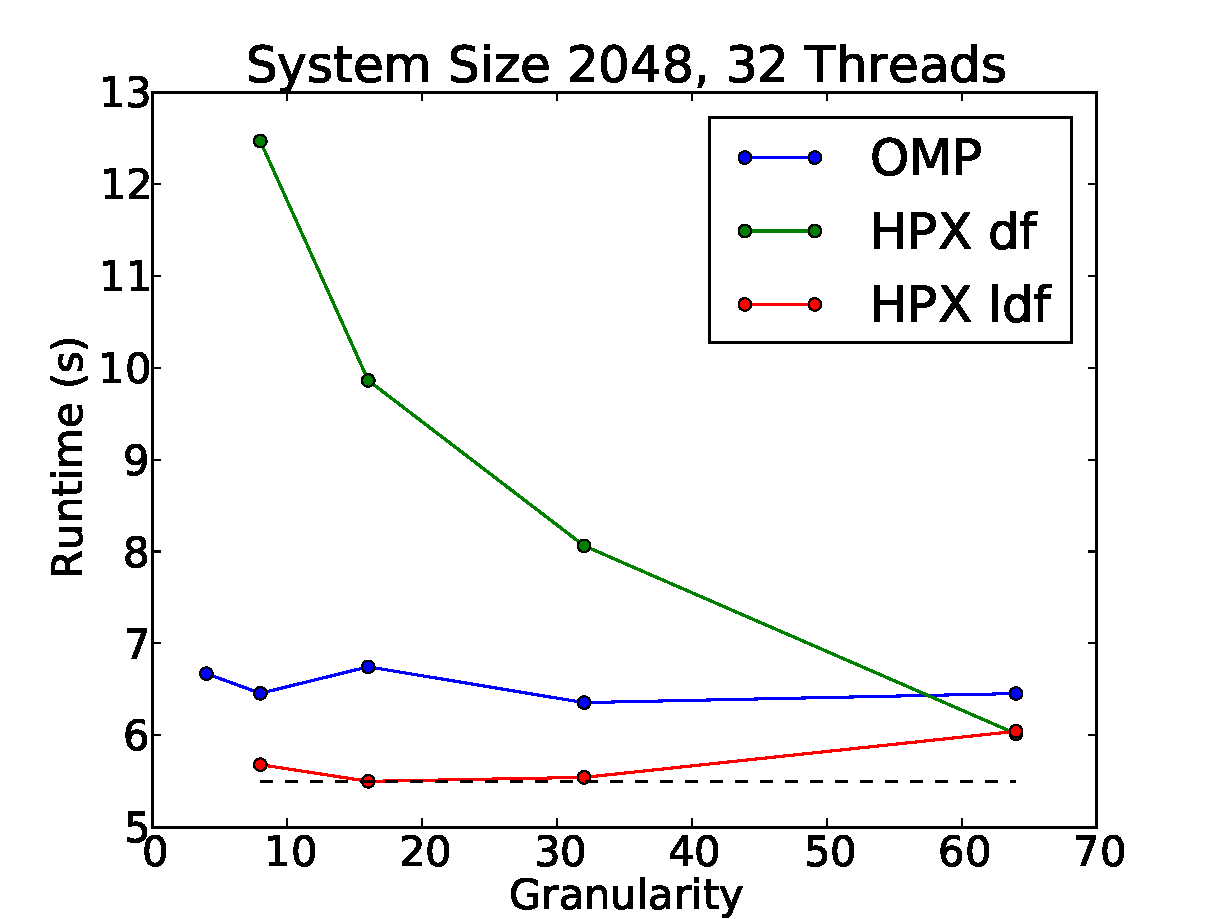
\includegraphics[width=\textwidth]{../plot/trillian_granularity_32.pdf}\hfill
  \caption{Granularity with 32 Threads.} 
  \label{fig:granularity_32}
 \end{subfigure}
 \caption{Granularity dependence of the run-time of the simulation on 16 (a) and 32 (b) Threads on a 4xOpteron6272 Machine (64 Cores). The granularity is the number of rows per task in the 2D simulation.}
\end{figure}

\begin{figure}
 \begin{subfigure}[b]{0.49\textwidth}
  \centering
  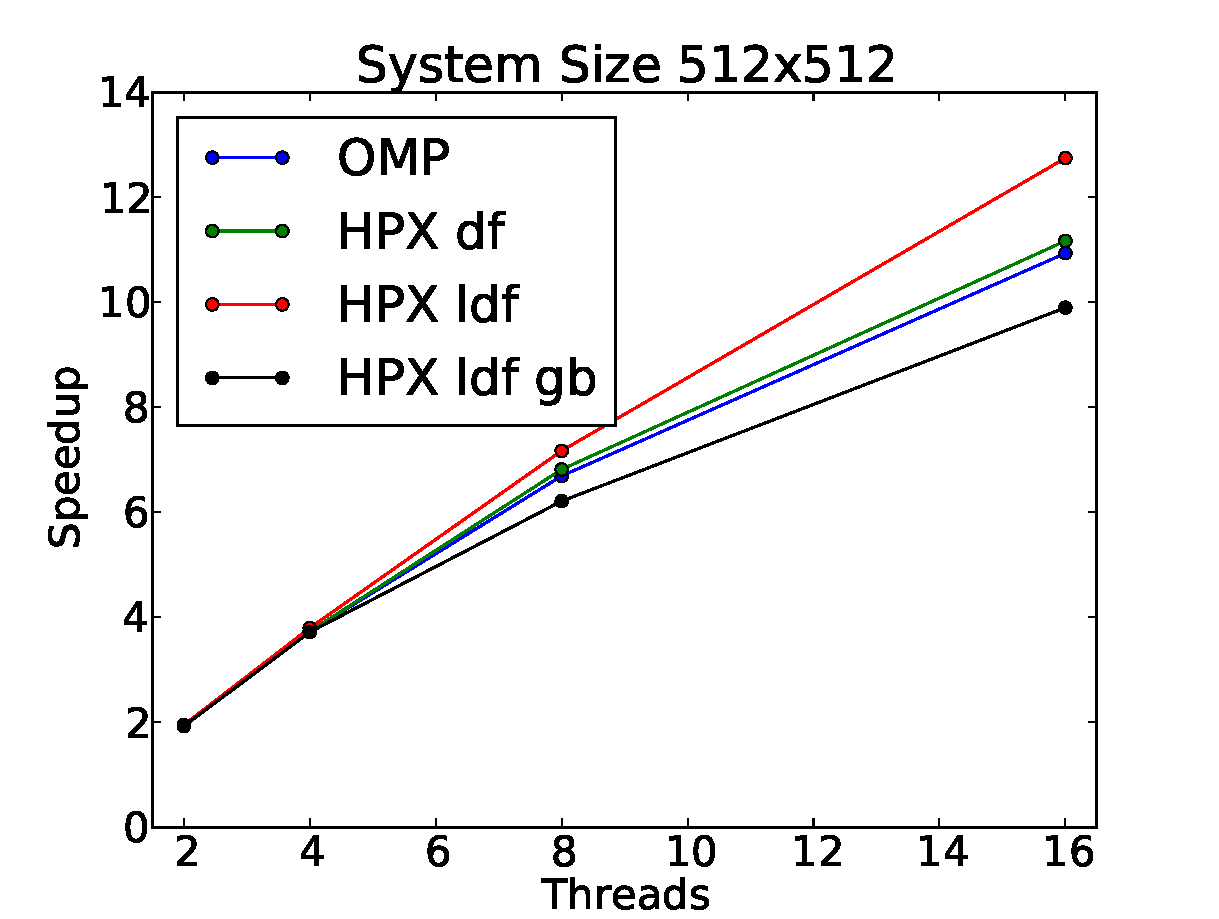
\includegraphics[width=\textwidth]{../plot/marvin_scaling_512.pdf}\hfill
  \caption{Performance with 512x512 lattice sites.} 
  \label{fig:scaling_marvin_512}
 \end{subfigure}
 \begin{subfigure}[b]{0.49\textwidth}
  \centering
  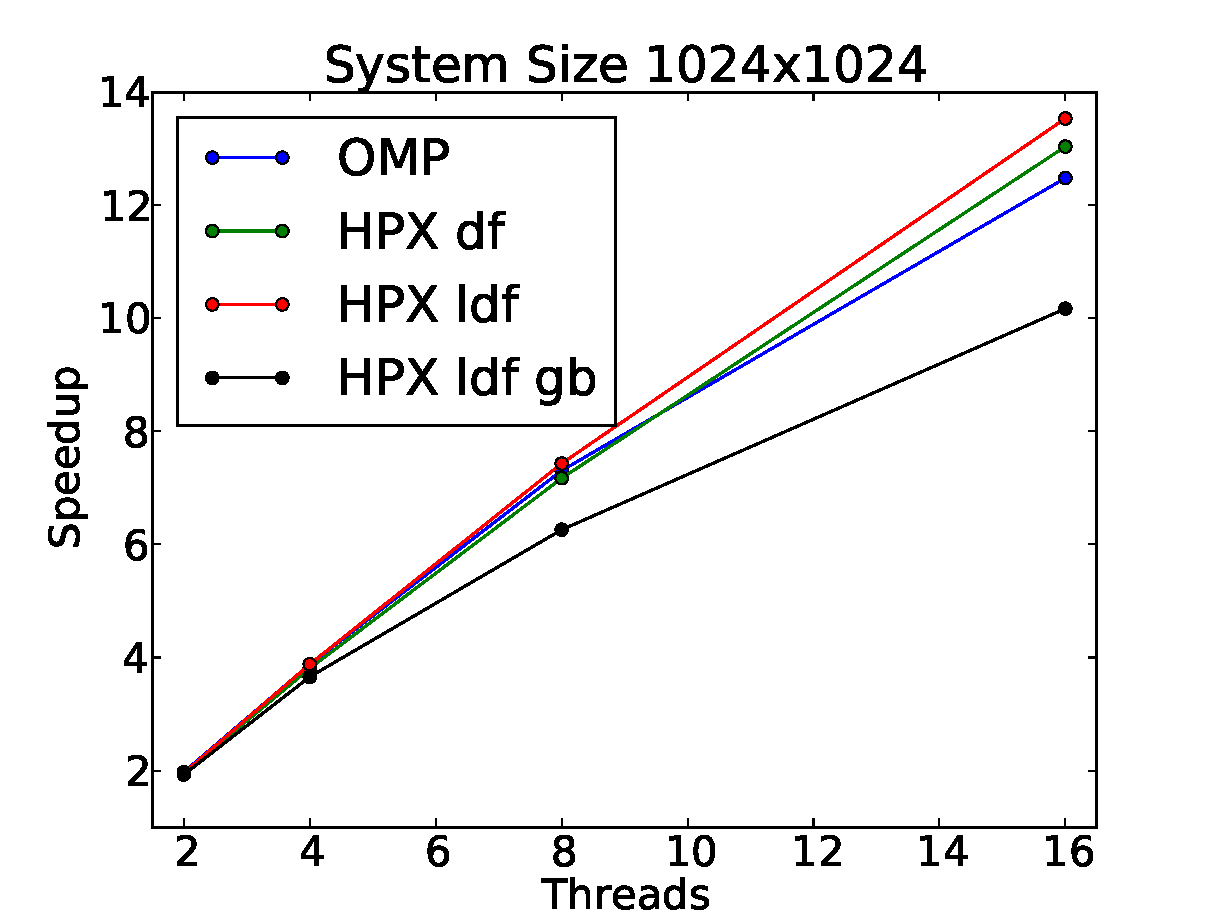
\includegraphics[width=\textwidth]{../plot/marvin_scaling_1024.pdf}\hfill
  \caption{Performance with 1024x1024 lattice sites.} 
  \label{fig:scaling_marvin_1024}
 \end{subfigure}
 \caption{Strong scaling for a system of size 512x512 (a) and 1024x1024(b) on a 2xXeonE5-2450 with 16 Cores (no Hyperthreading). The black curve (``HPX ldf gb'') represents the performance of a simulation using HPX local dataflows with additional global barriers.}
\end{figure}

\begin{figure}
 \begin{subfigure}[b]{0.49\textwidth}
  \centering
  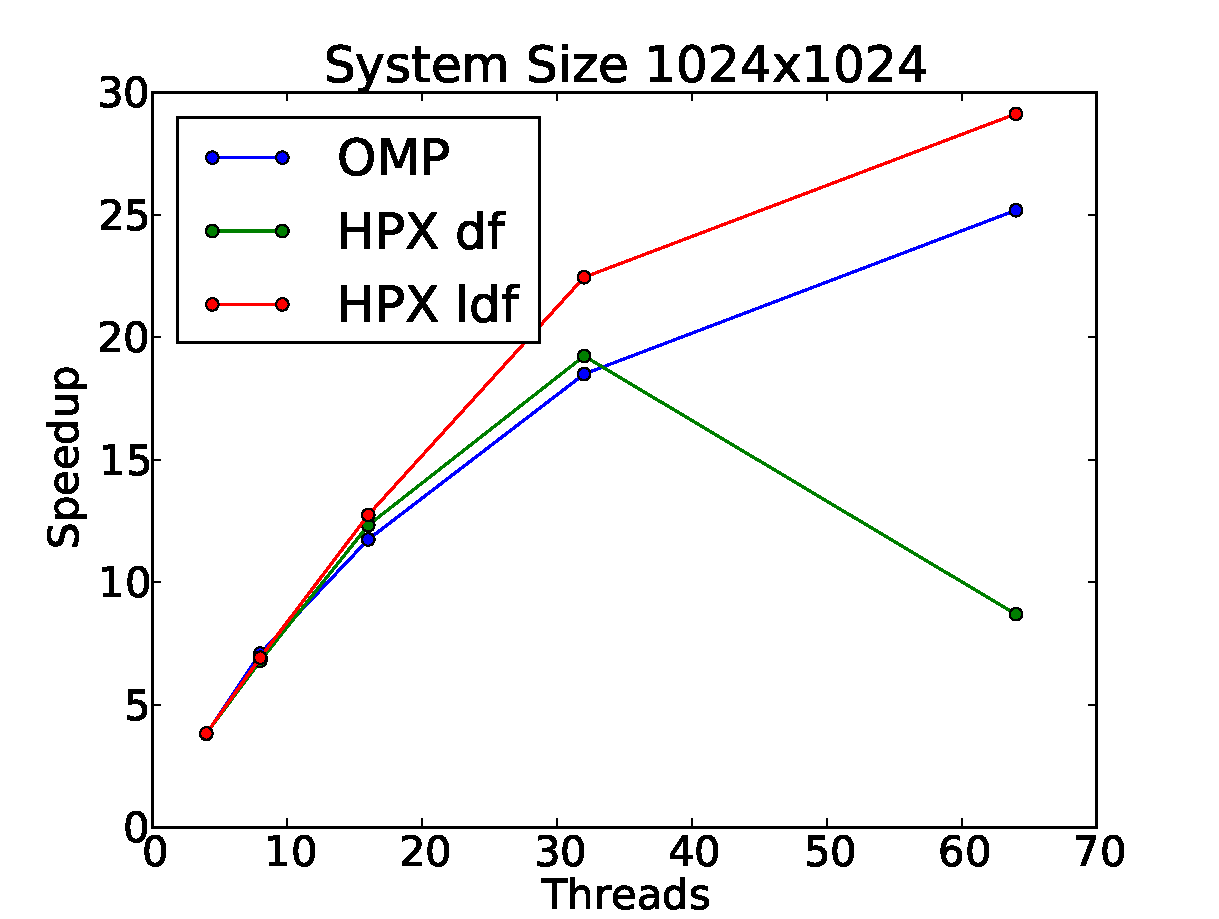
\includegraphics[width=\textwidth]{../plot/trillian_scaling_1024.pdf}\hfill
  \caption{Performance with 1024x1024 lattice sites.} 
  \label{fig:scaling_trillian_1024}
 \end{subfigure}
 \begin{subfigure}[b]{0.49\textwidth}
  \centering
  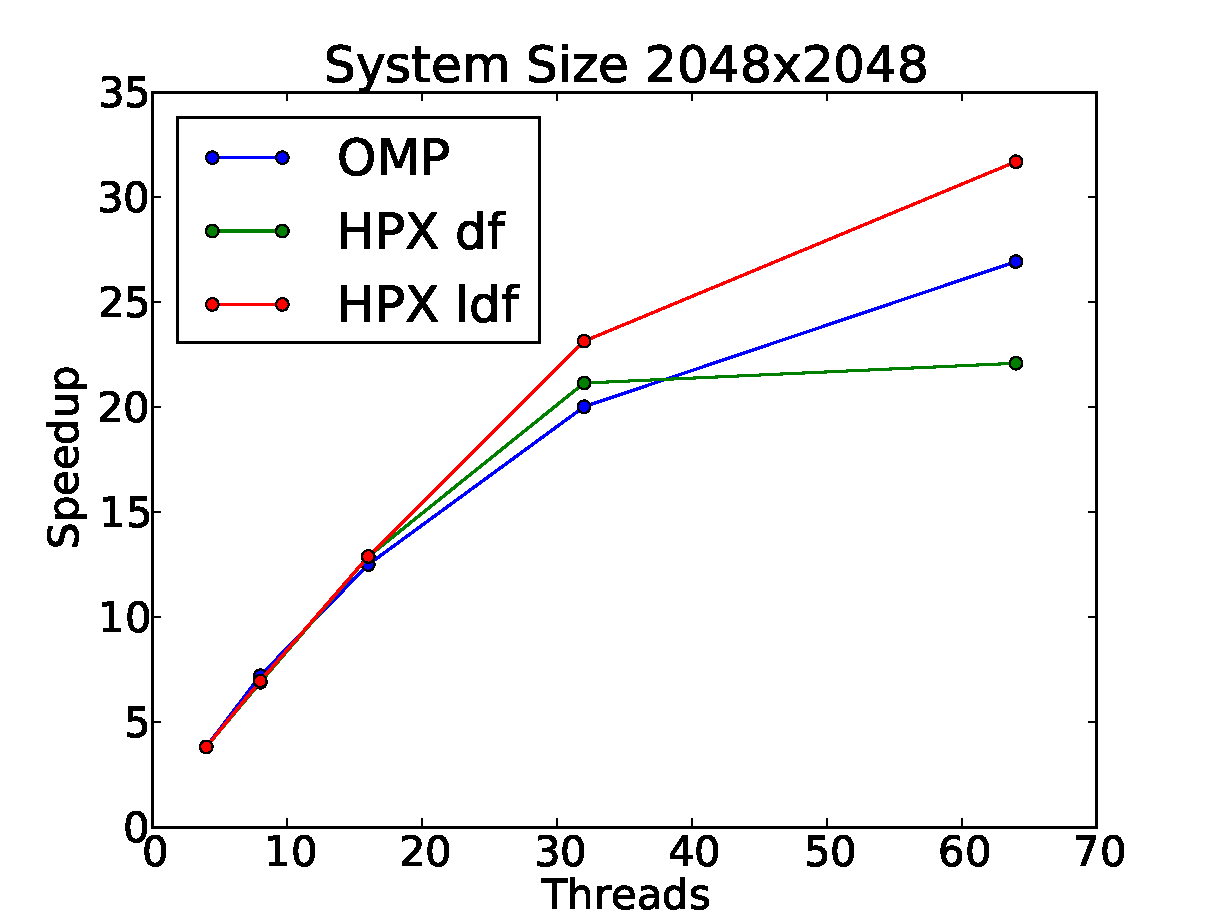
\includegraphics[width=\textwidth]{../plot/trillian_scaling_2048.pdf}\hfill
  \caption{Performance with 2048x2048 lattice sites.} 
  \label{fig:scaling_trillian_2048}
 \end{subfigure}
 \caption{Strong scaling for a system of size 1024x1024 (a) and 2048x2048(b) on a 4xOpteron6272 (64 Cores).}
\end{figure}

\end{document}          
